\input{configuration}

\title{Lecture 14 --- UNIX Processes and POSIX Threads (pthread) }

\author{Jeff Zarnett \\ \small \texttt{jzarnett@uwaterloo.ca}}
\institute{Department of Electrical and Computer Engineering \\
	University of Waterloo}
\date{\today}


\begin{document}

\begin{frame}
	\titlepage

\end{frame}


\begin{frame}
	\frametitle{UNIX Workflow}

	Parent spawns the child process with the \texttt{fork} system call.

	If waiting for the child process to finish, \texttt{wait}.\\
	\quad Alternatively, carry on.

	When the child process is finished, it returns a value with \texttt{exit}

	The parent gets this as the return value of \texttt{wait} and may proceed.
\end{frame}

\begin{frame}
	\frametitle{About \texttt{fork}}

	Note: \texttt{fork} creates a new process as a copy of itself.

	\begin{center}
		
\includegraphics[width=0.4\textwidth]{images/spiderman-2.jpg}
	\end{center}

	Both parent and child continue after that statement.

	The call \texttt{fork} can return a value:\\
	\quad A negative value means the fork failed.\\
	\quad A zero value means this process is the child.\\
	\quad A positive value: this is the parent; the value is the child \texttt{pid}.

\end{frame}

\begin{frame}
	\frametitle{After the \texttt{fork}, the \texttt{exec}}


	After the \texttt{fork}, one of the processes may use the \texttt{exec} system call.

	This will replace its memory space with a new program.

	There's no rule that says this must happen!\\
	\quad a child can continue to be a clone of its parent if it wishes.
	
\end{frame}

\begin{frame}
	\frametitle{After the \texttt{fork}, the \texttt{exec}}


	The \texttt{exec} invocation loads a binary file into memory \& starts execution.

	At this point, the programs can go their separate ways.

	Or the parent might want to wait for the child to finish.


\end{frame}

\begin{frame}[fragile]
	\frametitle{Putting it Together}

	{\scriptsize
		\begin{lstlisting}[language=C]
int main( int argc, char** argv ) {
  pid_t pid;
  int childStatus;

  /* fork a child process */
  pid = fork();
  
  if (pid < 0) { 
    /* error occurred */ 
    fprintf(stderr, "Fork Failed"); 
    return 1;
  
 } else if (pid == 0) {    
    /* child process */
    execlp("/bin/ls","ls",NULL);
    
  } else {    
    /* parent process */
    /* parent will wait for the child to complete */
    wait(&childStatus);
    printf("Child Complete with status: %i \n", childStatus);
    
  }
    
  return 0;
}
\end{lstlisting}
	}

\end{frame}

\begin{frame}[fragile]
	\frametitle{Code Output}

	Thus, the output is:
	\begin{verbatim}
jz@Freyja:~/fork$ ./fork 
fork   fork.c
Child Complete with status: 0
jz@Freyja:~/fork$ 
\end{verbatim}


\end{frame}

\begin{frame}
	\frametitle{Fork Visually}

	Or, to represent this visually:

	\begin{center}
		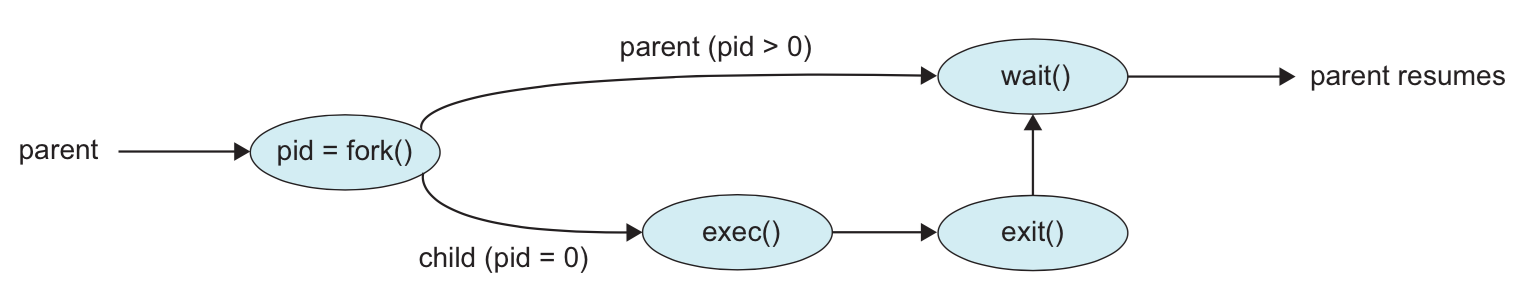
\includegraphics[width=\textwidth]{images/fork-syscall.png}
	\end{center}

\end{frame}

\begin{frame}
	\frametitle{Termination?}

	What about termination?

	On the assumption that the process is terminating normally and not being killed, the system call for that is \texttt{exit}.

	If the program itself has no explicit call to \texttt{exit}, the \texttt{return} statement at the end of \texttt{main} will have the same effect.

\end{frame}

\begin{frame}
	\frametitle{Termination?}

	The \texttt{wait} function also returns the process ID of the child.

	This is so that the parent can identify which of its children has terminated, though it is not used in this example.

\end{frame}

\begin{frame}
	\frametitle{After the \texttt{fork}}

	Afterwards, the system will need to choose which process is going to run:

	\begin{enumerate}
		\item The parent process. The child is in the ready to run state.
		\item The child process. The parent is in the ready to run state.
		\item Another process. Both parent and child are in the ready to run state.
	\end{enumerate}

\end{frame}


\begin{frame}
	\frametitle{Fork Design Problem}

	There is a task that can be split into parts 'A' and 'B'.

	Use \texttt{fork()} to create a child process.

	The child process should call function \texttt{execute\_B()} and return the result to the parent.

	The parent process should call \texttt{execute\_A()} and collect its result.

	The parent should then collect the result of the child using \texttt{wait()} and then produce the console output.

\end{frame}

\begin{frame}
	\frametitle{Fork Design Problem}
	If no errors occurred, \texttt{main} should return 0; otherwise it should return -1.

	If an error occurs, it should be reported to the console including the error number (e.g., ``Error 7 Occurred.'').

	If more than one error occurs, report both errors.

	If both functions return zero, it means all is well and the program should print ``Completed.'' to the console.

\end{frame}


\begin{frame}[fragile]
	\frametitle{Fork Design Solution}
	\begin{lstlisting}[language=C]
int main( int argc, char** argv ) {
  int child_result;
  int parent_result;

  pid_t pid = fork();
  if ( pid < 0 ) { /* Fork Failed */
    return -1;
  } else if ( pid == 0 ) { /* Child */
    return execute_B();
  } else { /* Parent */ 
    parent_result = execute_A();
    wait( &child_result );
  }
  
  if ( child_result == 0 && parent_result == 0 ) {
    printf( "Completed.\n" );
    return 0;
  }
  
  if ( child_result != 0 ) {
    printf( "Error %d Occurred.\n", child_result);
  }
  if ( parent_result != 0 ) {
    printf( "Error %d Occurred.\n", parent_result);
  }
  return -1;
}
\end{lstlisting}
\end{frame}

\begin{frame}
	\frametitle{Apr\`{e}s \texttt{fork}, le d\'{e}luge}

	A short digression on a denial of service attack: the ``fork bomb''.

	The idea is to call \texttt{fork} repeatedly.

	Keep doing this until the system crashes (or no work can get done).

	Exponential growth ($2^n$) processes after $n$ calls.

\end{frame}


\begin{frame}
	\frametitle{Fork Bomb}

	\begin{center}
		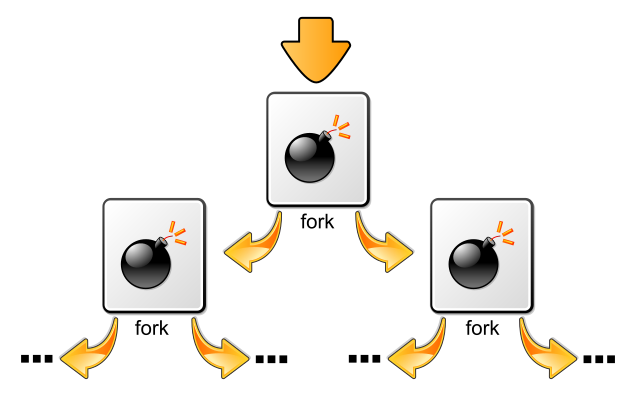
\includegraphics[width=\textwidth]{images/forkbomb.png}
	\end{center}
	\hfill Image Credit: Wikipedia user Dake

\end{frame}


\begin{frame}
	\frametitle{Apr\`{e}s \texttt{fork}, le d\'{e}luge}
	A system can be configured to defend against this.

	1. Limit total number of processes per user.

	2. Limit rate of process spawning.

	Note: do not attempt this on University computers!

\end{frame}


\begin{frame}
	\frametitle{The POSIX Thread}

	The term \texttt{pthread} refers to the POSIX standard (also known as the IEEE 1003.1c standard) that defines thread behaviour in UNIX.

Wait, why are we talking about this?!

This is an embedded systems type course...

\end{frame}

\begin{frame}
	\frametitle{The POSIX Thread}

The pthread model is very common and used all across industry.

Knowing about this might seriously help you get a co-op job.


It will also help you if you want to take ECE~459 in the future...\\
\quad Statistically, many of you do! 

\end{frame}


\begin{frame}
	\frametitle{The POSIX Thread}
	\begin{itemize}
		\item \texttt{pthread\_create}
		\item \texttt{pthread\_exit}
		\item \texttt{pthread\_join}
		\item \texttt{pthread\_detach}
		\item \texttt{pthread\_yield}
		\item \texttt{pthread\_attr\_init}
		\item \texttt{pthread\_attr\_destroy}
		\item \texttt{pthread\_cancel}
		\item \texttt{pthread\_testcancel}
	\end{itemize}

\end{frame}


\begin{frame}[fragile]
	\frametitle{Let's Make a New Thread}

	\begin{lstlisting}[language=C]
pthread_create( pthread_t *thread, 
		const pthread_attr_t * attr, 
		void *(*start_routine)( void * ), 
		void *arg);
\end{lstlisting}

	\texttt{thread}: a pointer to a \texttt{pthread} identifier and will be assigned a value when the thread is created.

	\texttt{attr}: attributes; may be \texttt{NULL} for defaults.

	\texttt{start\_routine}: the function the new thread is to run.

	\texttt{arg}: The argument passed to the routine we want to start.

\end{frame}


\begin{frame}[fragile]
	\frametitle{Start Routine}

	The type of \texttt{start\_routine} above is a function signature.

	Thus, the \texttt{pthread\_create} function has to be called with the name of a function matching that signature, such as:

	\begin{lstlisting}[language=C]
void* do_something( void* start_params )
\end{lstlisting}

	After creating a new thread, the process has two threads in it.

	Scheduling of the threads is up to the operating system.

\end{frame}


\begin{frame}[fragile]
	\frametitle{There Can Be Only One}

	C: it is normal to have a single return value from a function, but usually we can have multiple input parameters.

	But here we get only one of each?

	Define a \texttt{struct} for the argument and return type!

	\begin{lstlisting}[language=C]
void* function( void * void_arg ) {
  parameters_t *arguments = (parameters_t*) args;
  /* continue after this */
}
\end{lstlisting}

	We have to cast it inside the thread anyway...

	The caller of the \texttt{pthread\_create} function has to know what kind of argument is expected in the function being called.

\end{frame}


\begin{frame}
	\frametitle{Attributes}

	Attributes can be used to set whether a thread is detached or joinable, scheduling policy, etc.

	By default, new threads are usually joinable (that is to say, that some other thread can call \texttt{pthread\_join} on them).

	To prevent a thread from ever being joined, it can be created in the detached state (or use \texttt{pthread\_detach})

	For virtually all scenarios that we will consider in this course the default values will be fine.

\end{frame}


\begin{frame}
\frametitle{Threadception}

There is no mandatory hierarchy of threads.

\begin{center}
	\includegraphics[width=0.7\textwidth]{images/peerThreads.png}\\
	\hfill Image Credit: Blaise Barney
\end{center}

New threads can create other threads.

\end{frame}


\begin{frame}
	\frametitle{Off We Go}

	The thread executes its function, until of course it gets to the end.

	Usually, it will terminate with \texttt{pthread\_exit}.

	The use of \texttt{pthread\_exit} is not the only way that a thread may be terminated.

	Sometimes we want the thread to persist (hang around), but if we want to get a return value from the thread, then we need it to exit.

\end{frame}


\begin{frame}
	\frametitle{Nobody's Listening}

	If a thread has no return values, it can just \texttt{return NULL;}

	This will send \texttt{NULL} back to the thread that has joined it.

	If the function that is called as a task returns normally rather than calling the exit routine, the thread will still be terminated.

\end{frame}

\begin{frame}
	\frametitle{Oh... Guess You Didn't Need This After All}

	Another way a thread might terminate is if the \texttt{pthread\_cancel} function.\\
	\quad We'll come back to this topic in more detail soon.

	A thread may also be terminated indirectly: if the entire process is terminated or if \texttt{main} finishes first (without calling \texttt{pthread\_exit} itself).

	End \texttt{main} with \texttt{pthread\_exit} to automatically wait for all spawned threads.

\end{frame}


\begin{frame}
\frametitle{Report, Number One!}

\begin{center}
	\includegraphics[width=\textwidth]{images/pike-numberone.jpg}
\end{center}

\end{frame}


\begin{frame}[fragile]
	\frametitle{Report, Number One!}

	Like the \texttt{wait} system call, the \texttt{pthread\_join} is how we get a value out of the spawned thread:

	\begin{lstlisting}[language=C]
pthread_join( pthread_t thread, void** retval );
\end{lstlisting}

	\texttt{thread}: the thread you wish to join.

	\texttt{retval}: wait... two stars?

\end{frame}

\begin{frame}
	\frametitle{Gotta Play the Level Again, Only Got 2 Stars}

	What we are looking for is a pointer to a void pointer.

	That is, we are going to supply a pointer that the join function will update to be pointing to the value returned by that function.

	Typically we supply the address of a pointer.

	Maybe the example makes it clearer.
\end{frame}


\begin{frame}[fragile]
	\frametitle{Collecting Return Value}

	\begin{lstlisting}[language=C]
#include <stdlib.h>
#include <stdio.h>
#include <pthread.h>

void * run( void * argument ) { 
  char* a = (char*) argument;
  printf("Provided argument is %s!\n", a); 
  int * return_val = malloc( sizeof( int )); 
  *return_val = 99; 
  pthread_exit( return_val );
}

int main( int argc, char** argv ) { 
  if (argc != 2) {
      printf("Invalid args.\n");
      return -1; 
  }
  pthread_t t;
  void* vr; 
  
  pthread_create( &t, NULL, run, argv[1] );
  pthread_join( t, &vr );
  int* r = (int*) vr; 
  printf("The other thread returned %d.\n", *r);
  free( vr );
  pthread_exit( 0 );
}
\end{lstlisting}


\end{frame}


\begin{frame}
	\frametitle{Ah! Ah! Ah!}

	Next, we'll do an example where we don't use the return value of a thread, but do use attributes.

	For the sake of simplicity: we are just going to count!

	\begin{center}
		\includegraphics[width=0.6\textwidth]{images/countvoncount.jpg}
	\end{center}


\end{frame}



\begin{frame}[fragile]
	\frametitle{Slightly Larger Example}

	\begin{lstlisting}[language=C]
#include <pthread.h>
#include <stdio.h>

int sum; /* Shared Data */

void *runner(void *param);

int main( int argc, char **argv ) {
  pthread_t tid; /* the thread identifier */
  pthread_attr_t attr; /* set of thread attributes */

  if ( argc != 2 ) {
    fprintf(stderr,"usage: %s <integer value>\n", argv[0]);
    return -1;
  }
  if ( atoi( argv[1] ) < 0 ) {
    fprintf(stderr, "%d must be >= 0\n", atoi(argv[1]));
    return -1;
  }

  pthread_attr_init( &attr ); /* set the default attributes */
  pthread_create( &tid, &attr, runner, argv[1] ); /* create the thread */
  pthread_join( tid, NULL );
  printf( "sum = %d\n", sum );
  pthread_attr_destroy( &attr );
  pthread_exit( NULL );
}
\end{lstlisting}


\end{frame}

\begin{frame}[fragile]
	\frametitle{Slightly Larger Example}


	\begin{lstlisting}[language=C]
void *runner( void *param ) {
  int upper = atoi( param );
  sum = 0;
  for ( int i = 1; i <= upper; i++ ) {
    sum += i;
  }
  pthread_exit( 0 );
}
\end{lstlisting}

	In this example, both threads are sharing the global variable \texttt{sum}.

	Do we have coordination?

\end{frame}


\begin{frame}
	\frametitle{Coordination, Count to 10}
	Yes! The parent thread will join the newly-spawned thread (i.e., wait until it is finished) before it tries to print out the value.

	If it did not, the parent would print the sum early.

	Let's do a different take on that program.

	\begin{center}
		\includegraphics[width=0.6\textwidth]{images/sesamestreet.png}
	\end{center}

\end{frame}

\begin{frame}[fragile]
	\frametitle{Slightly Larger Example 2}

	\begin{lstlisting}[language=C]
#include <pthread.h>
#include <stdio.h>
#include <stdlib.h>

int sum = 0;

void* runner( void *param ) {
    int upper = atoi( param );
    for (int i = 1; i <= upper; i++ ) {
        sum += i;
    }
    pthread_exit( 0 );
}
\end{lstlisting}


\end{frame}

\begin{frame}[fragile]
	\frametitle{Slightly Larger Example 2}


	\begin{lstlisting}[language=C]
int main( int argc, char** argv ) {

    pthread_t tid[3];

    if ( argc != 2 ) {
        printf("An integer value is required as an argument.\n");
        return -1;
    }
    if ( atoi( argv[1]) < 0 ) {
        printf( "%d must be >= 0.\n", atoi(argv[1]) );
    }

    for ( int i = 0; i < 3; ++i ) {
        pthread_create( &tid[i], NULL, runner, argv[1] );
    }
    for ( int j = 0; j < 3; ++j ) {
        pthread_join( tid[j], NULL );
    }
    printf( "sum = %d.\n", sum );

    pthread_exit( 0 );
}
\end{lstlisting}

	What happens when we run this program?

\end{frame}


\begin{frame}
	\frametitle{Sometimes...}

	For very small values of the argument, nothing goes wrong.

	For a large number we get some strange and inconsistent results. Why?

	There are three threads that are modifying \texttt{sum}.

	Remember what we said about ``at the same time''? We have to come back to it.

\end{frame}

\begin{frame}
	\frametitle{Thread Cancellation}

	Thread cancellation is exactly what it sounds like: a running thread will be terminated before it has finished its work.

	The thread that we are going to cancel is called the \textit{target}.

	\begin{center}
		\includegraphics[width=0.5\textwidth]{images/canceled_flight.jpg}
	\end{center}

\end{frame}


\begin{frame}[fragile]
	\frametitle{Cancellation Type}

	\begin{enumerate}
		\item \textbf{Asynchronous Cancellation}
		\item \textbf{Deferred Cancellation}
	\end{enumerate}

	thread can declare its own cancellation type through the use of the function:
	\begin{lstlisting}[language=C]
pthread_setcanceltype( int type, int *oldtype )
\end{lstlisting}

	\texttt{type}: \texttt{PTHREAD\_CANCEL\_DEFERRED} or \texttt{PTHREAD\_CANCEL\_ASYNCHRONOUS}

	\texttt{oldtype}: previous state, if we care.

\end{frame}

\begin{frame}
	\frametitle{Send Cancellation}

	The pthread command to cancel a thread is \texttt{pthread\_cancel} and it takes one parameter (the thread identifier).

	To check if the current thread has been cancelled, the function call is \texttt{pthread\_testcancel} which takes no parameters.

	It's polite to check this, if it's a risk.

\end{frame}


\begin{frame}
	\frametitle{Cancellation Points}
	A  large number of functions are \alert{cancellation points}.

	That is, the POSIX specification requires there is an implicit check for cancellation when calling one of those functions.

	Even more are ``potential cancellation points'' -- maybe, maybe not?

\end{frame}



\begin{frame}
	\frametitle{Not Now!}
	Sometimes a thread could die before it has cleaned up.

	\begin{center}
		\includegraphics[width=0.5\textwidth]{images/tenthdoctor.jpeg}
	\end{center}

	This can leave memory allocated, things locked...

\end{frame}


\begin{frame}[fragile]
	\frametitle{Cleanup Handler}

	We can prevent this with cancellation handlers.

	The functions for cleaning up are:

	\begin{lstlisting}[language=C]
/* Register cleanup handler, with argument */
pthread_cleanup_push( void (*routine)(void*), void *argument );
/* Run if execute is non-zero */
pthread_cleanup_pop( int execute );
\end{lstlisting}

	The push function always needs to be paired with the pop function at the same level in your program (where level is defined by the curly braces).

\end{frame}


\begin{frame}[fragile]
	\frametitle{Don't You Forget About Me}

	Consider the following code:
	\begin{lstlisting}[language=C]
void* do_work( void* argument ) {
  struct job * j = malloc( sizeof( struct job ) );
  /* Do something useful with this structure */
  /* Actual work to do not shown */
  free( j );
  pthread_exit( NULL );
}
\end{lstlisting}


\end{frame}



\begin{frame}[fragile]
	\frametitle{Don't You Forget About me}

	\begin{lstlisting}[language=C]
void cleanup( void* mem ) {
  free( mem );
}

void* do_work( void* argument ) {
  struct job * j = malloc( sizeof( struct job ) );
  pthread_cleanup_push( cleanup, j );
  /* Do something useful with this structure */
  /* Actual work to do not shown */
  free( j );
  pthread_cleanup_pop( 0 ); /* Don't run */
  pthread_exit( NULL );
}
\end{lstlisting}


\end{frame}





\end{document}

